
\section{Signal Separation using Non Negative Matrix Factorization}

In this problem you will use NMF to separate a mixed signal into its component signals. Specifically, your goal is to separate music and speech sounds from a signal consisting of both.

The basic idea is that you will use NMF to first learn bases for speech and music. Then you will use the learned bases to separate out music and speech from a recording consisting of both.

Do the following processing steps.
\begin{enumerate}
    \item  In the directory \texttt{hw3materials/problem2} you will find \texttt{speech.wav} file. Read the speech signal and compute its spectrogram. You already did this in previous homework 1. Use the \texttt{stft} function followed by magnitude computation, as before;  
    \begin{lstlisting}
    % matlab 
    [s, fs] = audioread('filename');
    spectrogram = stft(s',2048,256,0,hann(2048))
    M = abs(spectrogram)
    \end{lstlisting}
    \begin{lstlisting}
    # python 
    spectrogram = librosa.stft(audio, n_fft=2048, hop_length=256, center=False, win_length=2048)
    M = abs(spectrogram)
    phase = spectrogram/(M + 2.2204e-16)
    \end{lstlisting}
    \item Do the same for \texttt{music.wav} file.
\end{enumerate}
If we call $M_m$ and $M_s$ the magnitude spectrum of the music and speech file respectively, then the dimensionality of both matrices should be $1025 \times 977$. 

\begin{figure}[h!]
    \centering
    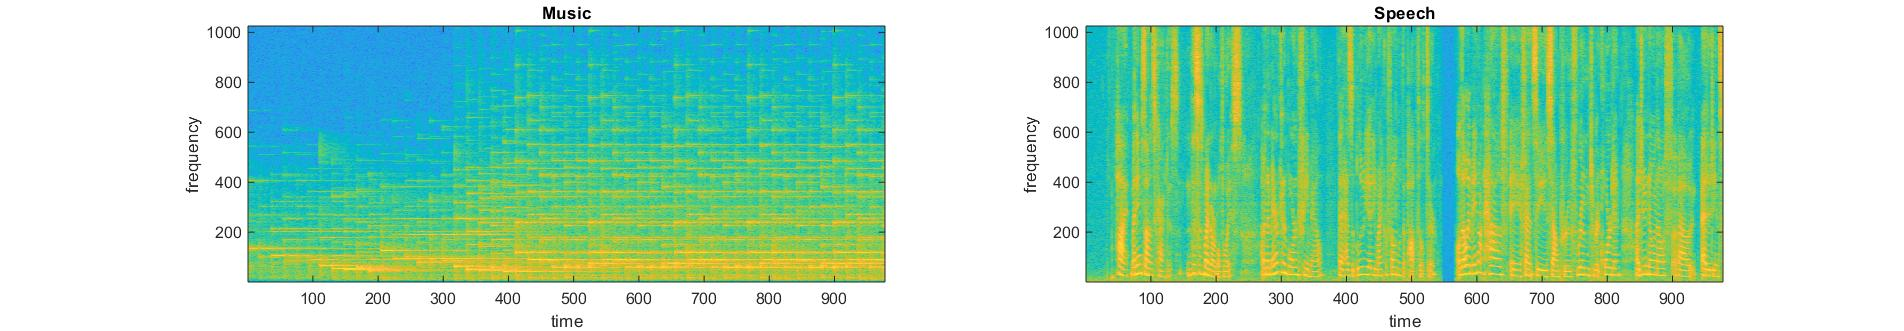
\includegraphics[trim ={6cm 0 0 0 }, scale=0.3]{figs/music_speech.jpg}
    \caption{Magnitude spectrum (in log scale) of files \texttt{music.wav} and \texttt{speech.wav}}
    \label{face_example}
\end{figure}


Now using the spectrograms for music $M_m$ and speech $M_s$ you are first going to learn bases, $B_m$ and $B_s$ for music and speech respectively. Therefore, we given the non-negative matrices $M_m$ and $M_s$, we need to find the non-negative matrices $B_m$, $W_m$, $B_s$ and $W_s$ such that
\begin{eqnarray}
    M_m & \approx & B_m \, W_m\\
    M_s & \approx & B_s \, \, W_s
\end{eqnarray}

 
\subsection{NMF Estimation: Learning Bases}

In this homework, given a non-negative matrix $M \in \mathbb{R}^{p \times q}$, we will consider the algorithm to estimate the non-negative matrices $B \in \mathbb{R}^{p \times k}$ and $W \in \mathbb{R}^{k \times q}$ that attempts to minimize the \textit{KL divergence} between $M$ and $BW$. The KL divergence between matrix $A$ and matrix $B$ is given by
\begin{eqnarray}
        D(A \,  || \, B) & = & \sum_{ij} \left( A_{ij} \log \left( \frac{A_{ij}}{B_{ij}} \right) - A_{ij} + B_{ij} \right) 
    \end{eqnarray}
Then, the algorithm that minimizes $D(M || BW)$ is the following:
\begin{itemize}
    \item Initialize $B$ and $W$ randomly.
    \item Iteratively update $B$ and $W$ using the following rule:
    \begin{eqnarray}
        B = B \, \otimes \, \frac{\left( \frac{M}{BW} \right) W^\top}{{\bf 1}_{p \times q} W^\top} \\
        W = W \, \otimes \, \frac{B^\top \left( \frac{M}{BW} \right)}{B^\top {\bf 1}_{p \times q}}
    \end{eqnarray}
    where $\otimes$ denotes component-wise matrix multiplication, $\frac{\; \cdot \;}{\cdot}$ denotes the component-wise matrix division, and ${\bf 1}_{p \times q}$ is the $p \times q$ matrix which each of its component is 1.
\end{itemize}

\begin{enumerate}
    \item Write the function \texttt{NMF\_train} which receives as inputs:
    \begin{itemize}
        \item \texttt{M}: a $p \times q$ non-negative matrix. 
        \item \texttt{B\_init}:  a $p \times k$ non-negative matrix. This matrix is the initial value of matrix $B$.
        \item \texttt{W\_init}: a $k \times q$ non-negative matrix. This matrix is the initial value of matrix $W$.
        \item \texttt{n\_iter}: a positive integer value. It determines the number of iterations of the algorithm.
    \end{itemize}
    Based on the algorithm previously described, the outputs of this function must be:
    \begin{itemize}
        \item \texttt{B}: a $p \times k$ non-negative matrix. 
        \item \texttt{W}: a $k \times q$ non-negative matrix.
    \end{itemize}
    \ul{Submit your code.}
    
    \item In the directory \texttt{hw3materials/problem2} you can find the files \texttt{Bm\_init.csv} and \texttt{Wm\_init.csv}. These files are matrices which must be used as initial condition to run your function \texttt{NMF\_train} over the magnitude spectrum of the music signal $M_m$. Consider values for \texttt{n\_iter} in $\{0, 50, 100, 150, 200, 250\}$. Run your function using these parameters and plot $D(M_m || B_mW_m)$ as function of \texttt{n\_iter}. \ul{Attach this plot to your report and write the value of $D(M_m||B_mW_m)$ for \texttt{n\_iter} $= 250$}.
    
    \item Similarly, you can also find in the directory \texttt{hw3materials/problem2} the files \texttt{Bs\_init.csv} and \texttt{Ws\_init.csv}. As before, these files are matrices which must be used as initial condition to run your function \texttt{NMF\_train} over the magnitude spectrum of the speech signal $M_s$. Repeat the previous task your this signal considering the same setting. \ul{Attach your plot to the report and write the value of $D(M_s||B_sW_s)$ for \texttt{n\_iter} $= 250$}. 
    
\end{enumerate}


\subsection{Signal Separation}

Now, using the bases you learned for speech and music, we will separate a signal which is a mix between a different speech signal and a music signal.

In the directory \texttt{hw3materials/problem2} you can find a file named \texttt{mixed.wav}. Compute its magnitude spectrum, that we will call $M_{\text{mixed}}$. The following figure visualize this matrix.

\begin{figure}[h!]
    \centering
    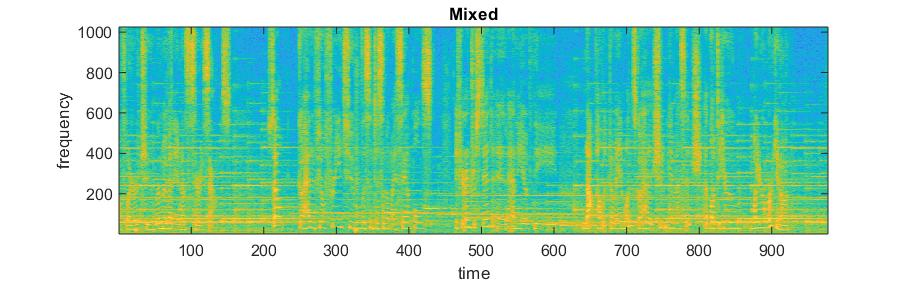
\includegraphics[trim ={0cm 0 0 0 }, scale=0.3]{figs/mixed.jpg}
    \caption{Magnitude spectrum (in log scale) of file \texttt{mixed.wav}}
\end{figure}



Our model considers that the bases we learned in the previous part are good enough to represent this audio file. More precisely, in this case, given $M_{\text{mixed}}$, $B_s$ and $B_m$, we need to learn the weights $W$ such that
\begin{eqnarray}
    M_{\text{mixed}} & \approx & [B_s \; B_m] W 
\end{eqnarray}
 In this equation, $[B_s \; B_m]$ represents the concatenation of the bases you already learned; so if $M_{\text{mixed}}$ is a $p \times q$ matrix, $[B_s \; B_m]$ is a $p \times 2k$ matrix. Moreover, the matrix $W$ gives us the contribution of each element in this \textit{new} set of bases. 
 To learn $W$ we can use the previous algorithm, but without updating the bases $B$ (we already know $B$).
 

\begin{enumerate}
    \item Write the function \texttt{separate\_signals} which receives as inputs:
    \begin{itemize}
        \item \texttt{M\_mixed}: a $p \times q$ non-negative matrix. 
        \item \texttt{B\_speech}:  a $p \times k$ non-negative matrix. This matrix is the bases you have to represent speech.
        \item \texttt{B\_music}: a $p \times k$ non-negative matrix. This matrix is the bases you have to represent music.
        \item \texttt{n\_iter}: a positive integer value. It determines the number of iterations of the algorithm.
    \end{itemize}
    The output of this function must be:
    \begin{itemize}
        \item \texttt{M\_speech\_rec}: a $p \times q$ non-negative matrix. It is the recovered speech magnitude spectrum.
        \item \texttt{M\_music\_rec}: a $p \times q$ non-negative matrix. It is the recovered music magnitude spectrum.
    \end{itemize}
    \ul{Submit your code}
    
    \item Using the bases you learned from the previous problem when you considered \texttt{n\_iter} $= 250$, apply your function \texttt{separate\_signals} using the magnitude spectrum of the mixed signal and taking \texttt{n\_iter} = 500. \ul{Submit your output as \texttt{M\_speech\_rec.csv} and \texttt{M\_music\_rec.csv}}.
    
    
    \item Now using the phase for the mixed signal along with reconstructed spectrograms, reconstruct time domain music and speech signals. You did this in homework 1 as well. You can use the \texttt{stft} function again to do this. Save the generated signals as \texttt{speech\_rec.wav} and \texttt{music\_rec.wav}. \ul{Submit these two files}.
    
    
\end{enumerate}
 













\iffalse

\section{Eigen Faces and Face Detection}

\subsection{Compute EigenFaces}

In the directory \texttt{hw2material/problem2} you can find a folder named \texttt{lfw1000}, which contains 1071 face images. Each of these images is a $64 \times 64$ gray scale image. The figure \ref{face_example} shows some examples.


\begin{figure}[h!]
    \centering
    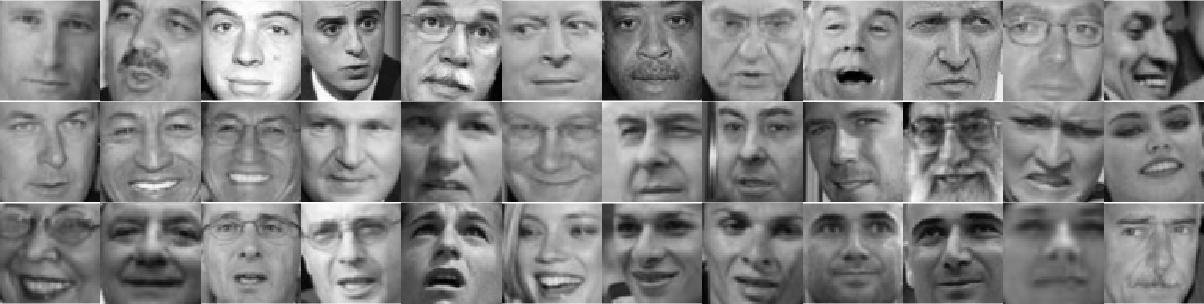
\includegraphics[scale=0.35]{figs/faces.jpg}
    \caption{Examples of face images.}
    \label{face_example}
\end{figure}


The matlab command to read an image is:
\begin{lstlisting}
image = double(imread(imagefile));
\end{lstlisting}
Note we are using \texttt{double()}. If you do not use it, matlab reads the data as \texttt{uint8} and some operations cannot be performed.


We consider that each face can be approximated by a linear combination of eigenfaces, this is, each face $F$ can be approximated as
\begin{equation}
  F & \approx & \omega_{F,1}E_1 + \omega_{F,2}E_2 +...+\omega_{F,k}E_k  
\end{equation}\\
where $E_i$ is the $i^{\text{th}}$ Eigen face and $\omega_{F,i}$ is the weight of the $i^{\text{th}}$ Eigen face, when composing face $F$. 

To learn eigen vectors, the collection of faces must be unravelled into a matrix. To unravel an image of any size, you can do the following:
\begin{lstlisting}
[nrows, ncolumns] = size(image);
image = image(:);
\end{lstlisting}
The first line above is used only to retain the size of the original image. We will need it to fold an
unravelled image back into a rectangular image. The second line converts the \texttt{nrows} $\times$ \texttt{ncolumns} image into
a single \texttt{nrows}$\cdot$\texttt{ncolums} $\times$ $1$ vector. 
To read in an entire collection of images, you can do the following:
\begin{lstlisting}
filenames = textread('FILE WITH LIST OF IMAGE FILE NAMES','%s');
nimages = length(filenames);
for i = 1:nimages
    image{i} = double(imread(filenames{i}));
end
\end{lstlisting}

To compose matrix from a collection of \texttt{k} images, the following matlab script can be employed (you can also do it your own way):
\begin{lstlisting}
X = [];
for i = 1:k
    X = [X image{i}(:)];
end
\end{lstlisting}

Eigen faces can be computed from \texttt{X}, which is an (\texttt{nrows} $\cdot$ \texttt{ncolumns}) $\times$ \texttt{nimages} matrix. There are two ways
to compute eigen faces; one is using eigen analysis and the other is by singular value decomposition (in matlab, you can use the commands \texttt{eig} or \texttt{svd}).

The eigen face will be in the form of a \texttt{nrows} $\cdot$ \texttt{ncolumns} $\times$ $1$ vector. To convert it to an image, you must
fold it into a rectangle of the right size. Matlab will do it for you with:
\begin{lstlisting}
eigenfaceimage = reshape(eigenfacevector, nrows, ncolumns);
\end{lstlisting}
\texttt{nrows} and \texttt{ncolumns} are the values obtained when you read the image. \texttt{eigenfacevector} is the eigen vector
obtained from the eigen analysis (or SVD).

\begin{enumerate}
    \item \textbf{First Eigen Face}. 
    
    Using these 1071 images, find the first eigen face and plot it in your report (you can use the matlab commnad \texttt{imagesc}). \ul{Submit the first eigen face as a $4096 \times 1$ vector in a file named \texttt{eigenface.csv}}
    
    \item \textbf{Reconstruction Error}. 
    
    Given a face $F$ and the first $k$ eigenfaces, we can compute its reconstruction error as
    \begin{equation}
     \mathcal{E}(F \; ; \; E_1,...,E_k) & = & \left\| F - \sum_{i=1}^k \omega_{F,i} E_i \right\|^2_2
    \end{equation}
    
    Then, if we have $N$ faces, the mean reconstruction error is given by
    \begin{equation}
        \frac{1}{N} \sum_{j=1}^N \mathcal{E}(F_j \; ; \; E_1,...,E_k)
    \end{equation}
     
    Using the 1071 provided images, plot the mean reconstruction error as function of $k$. Consider $k$ from 1 to 100. \ul{Attach this plot to your report. Report the mean reconstruction error using $k=100$}. 
    
        
\end{enumerate}

\subsection{Adaboost Implementation}

In class we saw that Adaboost allows us to train a strong classifier combining weak classifiers, taking the following form:
\begin{eqnarray}
    F({\bf x}) & = & \sum_{t=1}^T \alpha_t \, h_t({\bf x}) \label{score}\\
    H({\bf x}) & = & \text{sign} \left( F({\bf x}) \right)
\end{eqnarray}
where $h_t$ is the $t$-th weak classifier and $\alpha_t$ the weight computed in the training phase. In this part, you have to implement your own version of Adaboost.
\begin{enumerate}
    \item Write the function \texttt{adaboost\_train} which receives as inputs:
    \begin{itemize}
        \item \texttt{X\_tr}: a $N \times M$ matrix, where each row corresponds to a data sample with M dimensions. This is the training data.
        \item \texttt{Y\_tr}: a $N  \times 1$ matrix, which contains 1s and -1s only. This vector defines the class label. The $i$ component is the class corresponding to the $i$-th row of \texttt{X\_tr}.
        \item \texttt{T}: a integer number. It defines the number of weak classifiers to use.
    \end{itemize}
    The output of this function must be \texttt{model}. This can be any data structure that contains all the information you need to make the inference. If you plan to work with matlab, we recommend to use \href{https://www.mathworks.com/help/matlab/structures.html}{structures}.
    
    \item Write the function \texttt{adaboost\_predict} which receives as inputs:
    \begin{itemize}
        \item \texttt{model}: this is the output obtained from function \texttt{adaboost\_train}
        \item \texttt{X\_te}: a $P \times M$ matrix, where each row corresponds to a data sample with $M$ dimensions.
    \end{itemize}
    The output of this function must be:
    \begin{itemize}
        \item \texttt{pred}: a $P \times 1$ vector, where each component is a real number. The $i$-th component is the prediction score $F$ (equation \ref{score}) for the $i$-th row of \texttt{X\_te}. Note that the actual prediction will be \texttt{sign(pred)}.
    \end{itemize}
    \ul{Submit your code}.
\end{enumerate}


\subsection{Training Adaboost}
In this part, you have to use your implementation of Adaboost.

In the directory hw2materials/problem2/ you can also find 2 folders: \texttt{train} and \texttt{test}. In each of these
you can find two folders: \texttt{face} and \texttt{non-face}. In the folder \texttt{face} there are pictures of faces, while in the
folder \texttt{non-face} there are non faces images. Each of these images is a $19 \times 19$ gray scale image.




We use the eigenfaces to represent each image as a real value vector. As we discuss in class, we can project the image $I$ on the eigenface $E_i$ and use the corresponding weight $\omega_{I,i}$ as one component of this representation. Formally, an image $I$ is represented as follows
\begin{eqnarray}
    \mathcal{R}(I \, ; \, E_1, ..., E_k) & = & \left( \begin{array}{c} \omega_{I,1} \\ \omega_{I,2} \\ \vdots \\ \omega_{I,k} \end{array} \right)
\end{eqnarray}
To do this, we need that the image and the eigen faces have the same size. 
\begin{enumerate}
    \item Rescale the images from folder \texttt{lfw1000} to a $19 \times 19$ size. You can use the command 
    \begin{lstlisting}
    image = imresize(image,[19,19]);
    \end{lstlisting}
    Then, compute new $19 \times 19$ eigenfaces using this new set.
    
    \item Considering the first $k = 10$ eigenfaces, for every image compute the projection to each eigen face, and use these values as features for your classifier. Thus, for each image you have to compute a vector with 10 components. 
    To define \texttt{Y\_tr}, consider 1 for face and -1 for non-face. Train your model using the representation of the images in the \texttt{train} folder and using different values of \texttt{T} (10, 50, 100, 150, 200). Plot your classification errors both in the training and testing set as a function of \texttt{T}. \ul{Attach this plot to your report}.

    \item Repeat and report the previous step taking $k = 30$ and $k = 50$. Is there any improvement? \ul{Attach the corresponding plots to your report}.
\end{enumerate}

\subsection{Face Detector}
The task of face detector is finding the location of faces in a give image. As we learned from the class, a typical face detector has following steps.

\begin{enumerate}
    \item Convert the given image to gray scale and rescale it  to different sizes.
    
    \item For each scale, use a face/non-face classifier to ``scan" the images in a sliding window manner. Here the classifier is trained in section 2.3. Note that we use the predicted score (equation \ref{score}) instead of the predicted label of the AdaBoost classifier. With the response score for each window, we have a score map for each scale. Eventually we have a bunch of score maps in different scales. Each score in the map indicates the possibility that the patch in this window is a face. The windows are also called bounding box.
    \item Find the local maximums in the score map and compare them to a threshold. Remove the ones with scores less than threshold. 
    \item Compute the corresponding bounding boxes based on the scores. Fuse the results from score maps of different scales.
    \item Use non-maximum suppression (NMS) to find the potential bounding boxes. NMS is a post-processing algorithm that merges all bounding boxes that belong to the same face.
\end{enumerate}


\begin{figure}[h!]
    \centering
    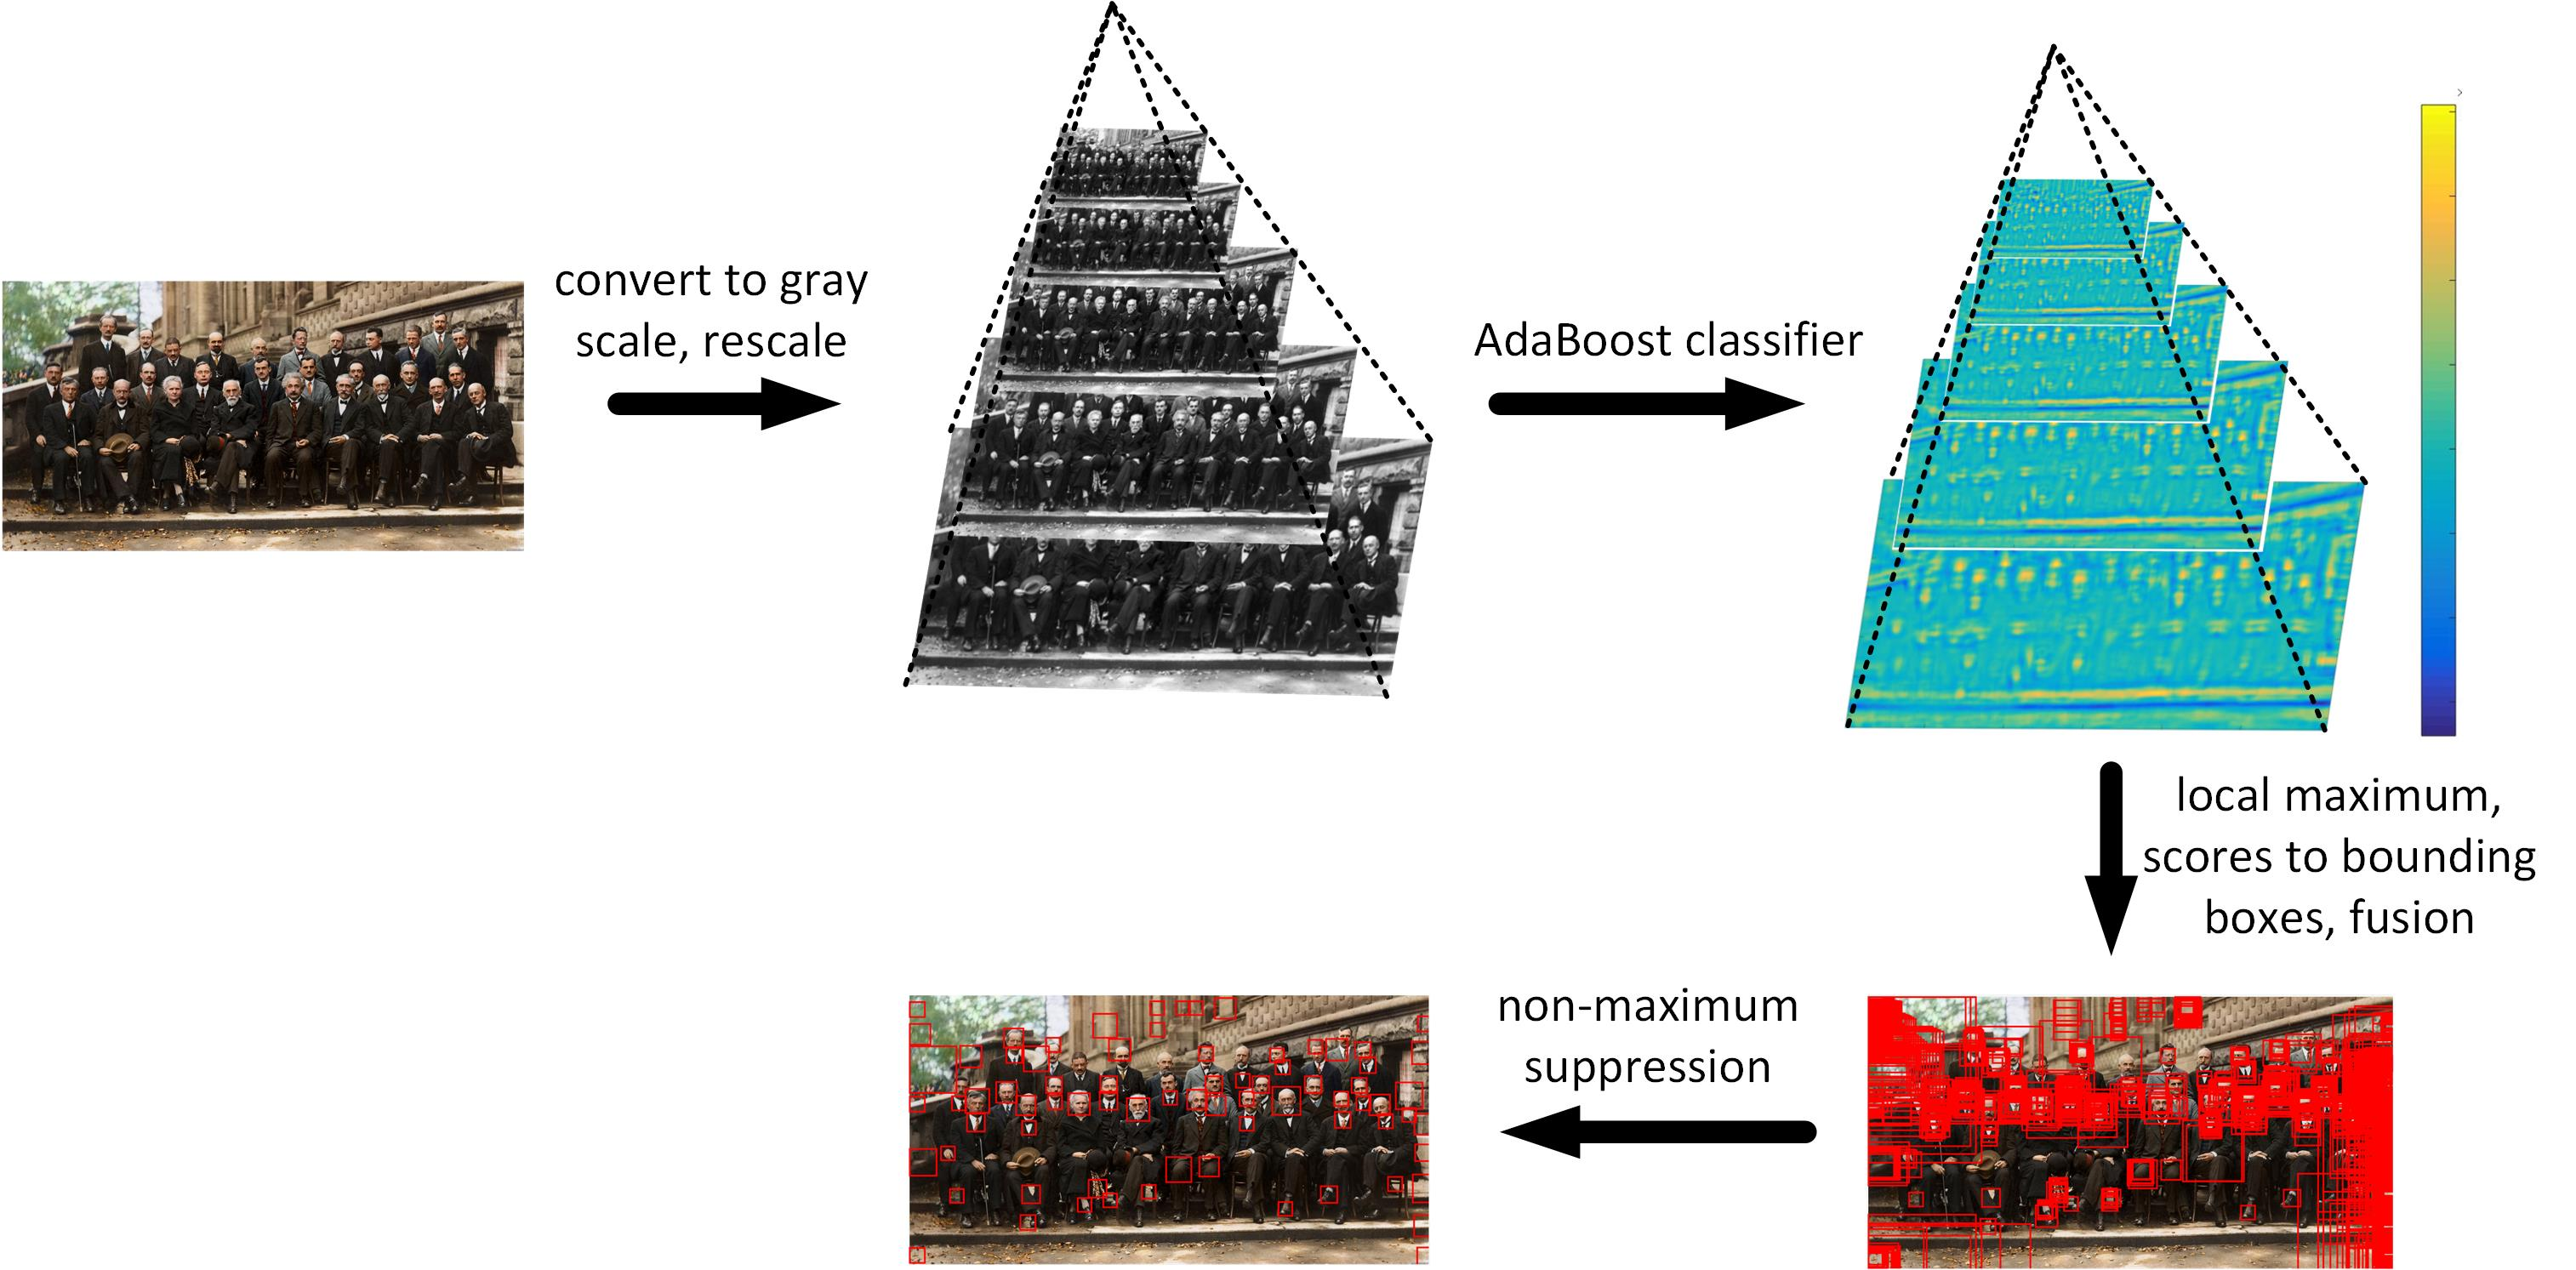
\includegraphics[scale=0.3]{figs/pipeline.jpg}
    \caption{Pipeline for Face Detection.}
    \label{pipeline}
\end{figure}

It would be more intuitive in fig. \ref{pipeline}. In this homework, step 3 and 5 is provided through two matlab functions that you can find in \texttt{h2materials/problem2/utils}:
\begin{itemize}
    \item \texttt{get\_localmax}: This function return the locations which may have a face. The candidate locations must be the local maximum, and their scores are greater than a pre-defined threshold.
    \item \texttt{nms}: This function implements non maximum suppression (NMS), a post-processing algorithm for merging the bounding boxes that belong to the same face. For each loop, it takes a bounding box with highest score, and removes the rest of bounding boxes that overlap with it.
\end{itemize}

Details about inputs and outputs can be found on the corresponding files.


You need to \ul{implement step 1, step 2, and step 4, and build the entire face detection system.} 

To test your system, 4 images are provided in the directory \texttt{hw2materials/problem2/photos}. \ul{Using these images, show your best results and the running times in the report.} You are allowed to tune different parameters (number of eigenfaces, number of weak learners, threshold, etc). The result should be in the form of image with the predicted bounding boxes.

\fi
